\section{Introduction}
\subsection{Présentation générale}
Les manœuvres de stationnement pouvant être parfois difficiles pour certains conducteurs, les constructeurs
automobiles proposent depuis maintenant quelques années une option de stationnement automatique sur leurs
véhicules. Cette fonctionnalité est permise par un système embarqué qui permet l’automatisation d’une manœuvre de stationnement (pour des places en créneau, épi ou bataille).

\begin{figure}[H]
\centering
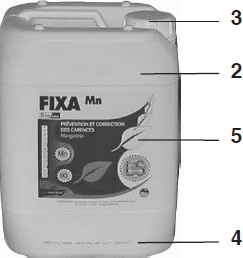
\includegraphics[width=.45\linewidth]{fig_00.png}
%\caption{ \label{fig_}}
\end{figure}

L’intervention du système de stationnement se fait sur la direction du véhicule : le système gère automatiquement l’orientation des roues avant du véhicule (et donc celle du volant). Quant au conducteur, il contrôle le
déplacement du véhicule (marche avant ou arrière) et la vitesse du véhicule avec la pédale d’accélération. Cette
vitesse est limitée et est supposée constante pendant la manœuvre.
Ce type d’aide au stationnement permet une meilleure précision de la manœuvre et un stationnement dans un
espace plus restreint en optimisant l’insertion du véhicule dans une place libre.
Les principaux éléments technologiques entrant en jeu dans cette automatisation des manœuvres de stationnement sont : le calculateur du véhicule, la motorisation de la direction du véhicule et les capteurs à ultrasons (généralement entre 4 et 6 capteurs à l’avant et à l’arrière).

\begin{figure}[H]
\centering
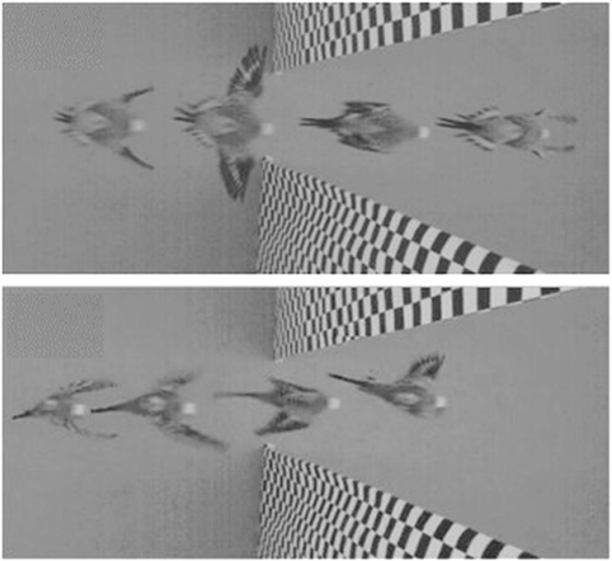
\includegraphics[width=.45\linewidth]{fig_01.png}
\caption{Détection par ultrasons (4 capteurs) \label{fig_01}}
\end{figure}

La procédure d’insertion automatisée du véhicule dans une place de stationnement, du point de vue du conducteur, est décrite par la \autoref{fig_02} dans le cas d’une insertion en créneau parfaitement exécuté. Sur la figure, le
véhicule est équipé de 4 capteurs à ultrasons à l’avant et à l’arrière.

Lorsque le conducteur voit une place libre devant lui, il active le stationnement automatique par l’appui d’un
bouton dédié sur son tableau de bord. La voiture est parallèle au trottoir et se déplace dans le sens normal de
la marche (repère 1 \autoref{fig_02}).

Le déclenchement du stationnement automatique a pour conséquence la détection de l’emplacement libre par
les capteurs ultrasons équipant la voiture lorsque celle-ci se déplace (repère 2 \autoref{fig_02}).
Si la place de stationnement est suffisamment longue et profonde alors le conducteur est prévenu que la manœuvre
est possible par un voyant lumineux situé sur son tableau de bord. Le conducteur doit alors arrêter son véhicule
(repère 3 \autoref{fig_02}) et mettre la boite de vitesses au point mort (position neutre).


\begin{figure}[H]
\centering
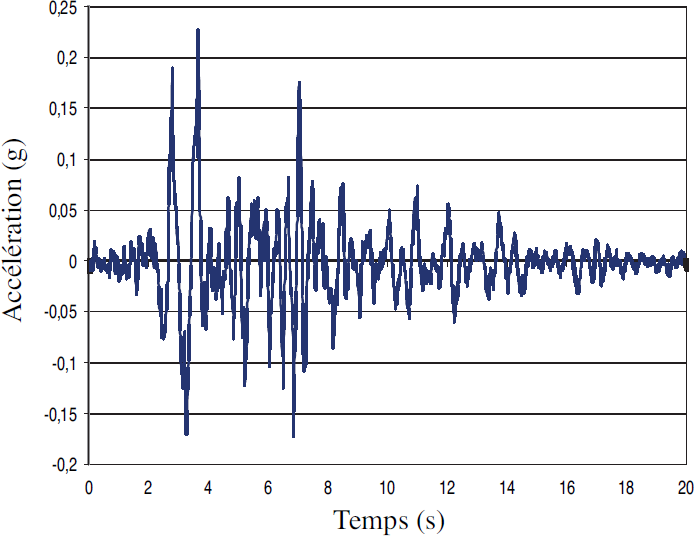
\includegraphics[width=.45\linewidth]{fig_02.png}
\caption{Manoeuvre d’insertion en créneau dans une place de stationnement \label{fig_02}}
\end{figure}

Un signal sur le tableau de bord invite alors le conducteur à passer la marche arrière et à appuyer sur la pédale
d’accélération afin que le véhicule commence la manœuvre (repères 4 et 5 \autoref{fig_02}). Pendant la manœuvre le
conducteur ne touche pas le volant.
Le processus d’automatisation de l’insertion du véhicule dans une place de stationnement en créneau suit un
algorithme dont l’action dépend du type de manœuvre, de l’espace de stationnement et de la géométrie du
véhicule. Cet algorithme gère :
\begin{itemize}
\item la détection d’une place libre suffisamment longue et profonde pour la manœuvre ;
\item le calcul de la trajectoire à suivre ;
\item la commande de la direction du véhicule.
\end{itemize}
Les exigences que le système de stationnement doit respecter sont décrites en figure \autoref{fig_26}.

\subsection{Problématique et organisation de l’étude}
Lors d’un stationnement en créneau, c’est la phase d’insertion du véhicule dans la place envisagée qui va
conditionner la réussite du stationnement et le nombre de manœuvres permettant d’atteindre une position
correcte de stationnement.

\begin{obj}
L’étude proposée a pour objectif de définir et de valider les conditions et les modèles à implanter dans
un algorithme de stationnement automatique afin qu’une manœuvre d’insertion de type créneau dans
une place de stationnement soit réussie et qu’elle atteigne les niveaux de performance attendus.
\end{obj}

L’étude est limitée à une manœuvre en créneau dont la position finale est définie repère numéro 5 sur la \autoref{fig_02}.
La manœuvre d’insertion en stationnement doit être réalisée en une fois. Si l’insertion est réussie alors la position
finale de stationnement sera, dans un second temps, facilement atteinte par une légère avance du véhicule pour
être centré dans la place de stationnement.

Dans un premier temps l’étude portera sur le stationnement automatique d’un véhicule réel. Le travail mené en
début de sujet pour un véhicule réel pouvant être transposé (à l’échelle près) à tout type de véhicule roulant,
le support technique de l’étude sera dans un second temps une voiture radio commandée (elle sera présentée
ultérieurement dans l’étude). Ce choix est justifié par le fait qu’il n’est pas possible de réaliser des essais sur un
véhicule réel et que les choix technologiques de la commande de direction ne sont pas rendus accessibles par les
constructeurs automobiles.


\section{Détection de l’environnement et prédiction de la trajectoire de
stationnement}

La phase pendant laquelle le véhicule circule parallèlement à une place libre est primordiale car elle correspond
à la phase de détection de l’emplacement de stationnement. Cette détection doit permettre de vérifier la compatibilité de l’emplacement détecté avec la manœuvre automatisée et d’identifier dans l’environnement du véhicule
des repères géométriques à partir desquels l’algorithme pourra établir la trajectoire à suivre.
Ces deux tâches sont possibles grâce aux capteurs de proximité à ultrasons équipant le véhicule (\autoref{fig_02}) et à
l’exploitation de leurs signaux.

\begin{obj}
Les objectifs de cette partie sont de déterminer les conditions à implanter dans l’algorithme de stationnement pour la validation d’une place libre et de caractériser la géométrie de la trajectoire à
suivre pour mener avec succès la manœuvre de stationnement. Cette trajectoire servira de consigne à
l’algorithme pour son action sur la direction du véhicule.
\end{obj}

\subsection{Détection et caractérisation d’une place libre (exigence 1.4)}
\begin{obj}
L’objectif est de caractériser les conditions définissant une place compatible avec la manœuvre de
stationnement.
\end{obj}

Lors du fonctionnement du véhicule tous les capteurs sont actifs, mais tous ne sont pas forcément exploités
pour la manœuvre automatique. Ainsi on distingue les capteurs dont les signaux peuvent être exploités par
l’algorithme de stationnement et ceux dont le signal sera exploité pour la sécurité (des passagers, des autres
usagers de la route et des piétons lors de la manœuvre du véhicule).

\question{À partir du diagramme des exigences (\autoref{fig_26}) et de la \autoref{fig_02}, identifier le ou les capteurs à ultrasons pouvant participer au respect de l’exigence 1.4. Faire de même pour l’exigence 1.6.1.}

Dans la réalité, le signal du capteur latéral côté passager (capteur a \autoref{fig_03}) est suffisant pour détecter une
place de stationnement suffisamment spacieuse. Le signal fourni par le capteur a va permettre de savoir si la
place de stationnement envisagée par le conducteur est compatible avec la manœuvre, mais va aussi permettre
de définir certains repères géométriques de l’environnement. Ces repères géométriques vont servir de référence
pour l’élaboration de la trajectoire à suivre pour réaliser le stationnement en créneau.


\begin{figure}[H]
\centering
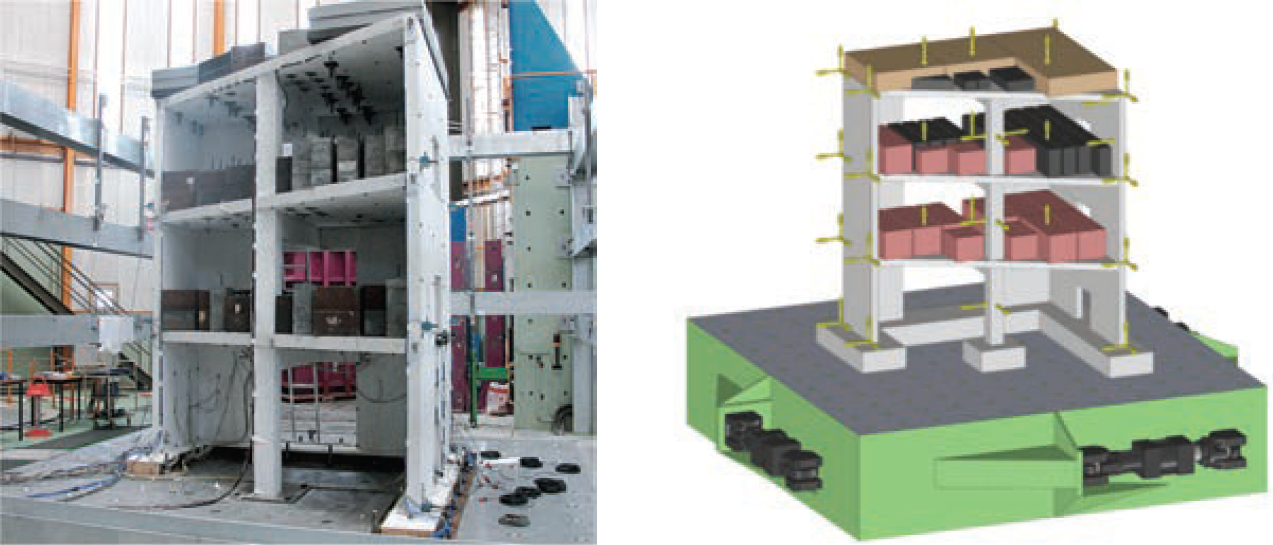
\includegraphics[width=.45\linewidth]{fig_03.png}
\caption{Phase de détection d’une place libre \label{fig_03}}
\end{figure}

Le type de capteur utilisé est un capteur de proximité à ultrasons (\autoref{fig_04}). Ce type de capteur possède une
membrane qui émet une onde ultrasonore par vibrations. La distance $d$ entre un capteur et un obstacle est
déduite du temps $T_e$ d’aller et retour de l’onde qui est réfléchie par l’obstacle puisque la vitesse du son dans
l’air est connue : $V_s = \SI{340}{m.s^{-1}}$.

\begin{figure}[H]
\centering
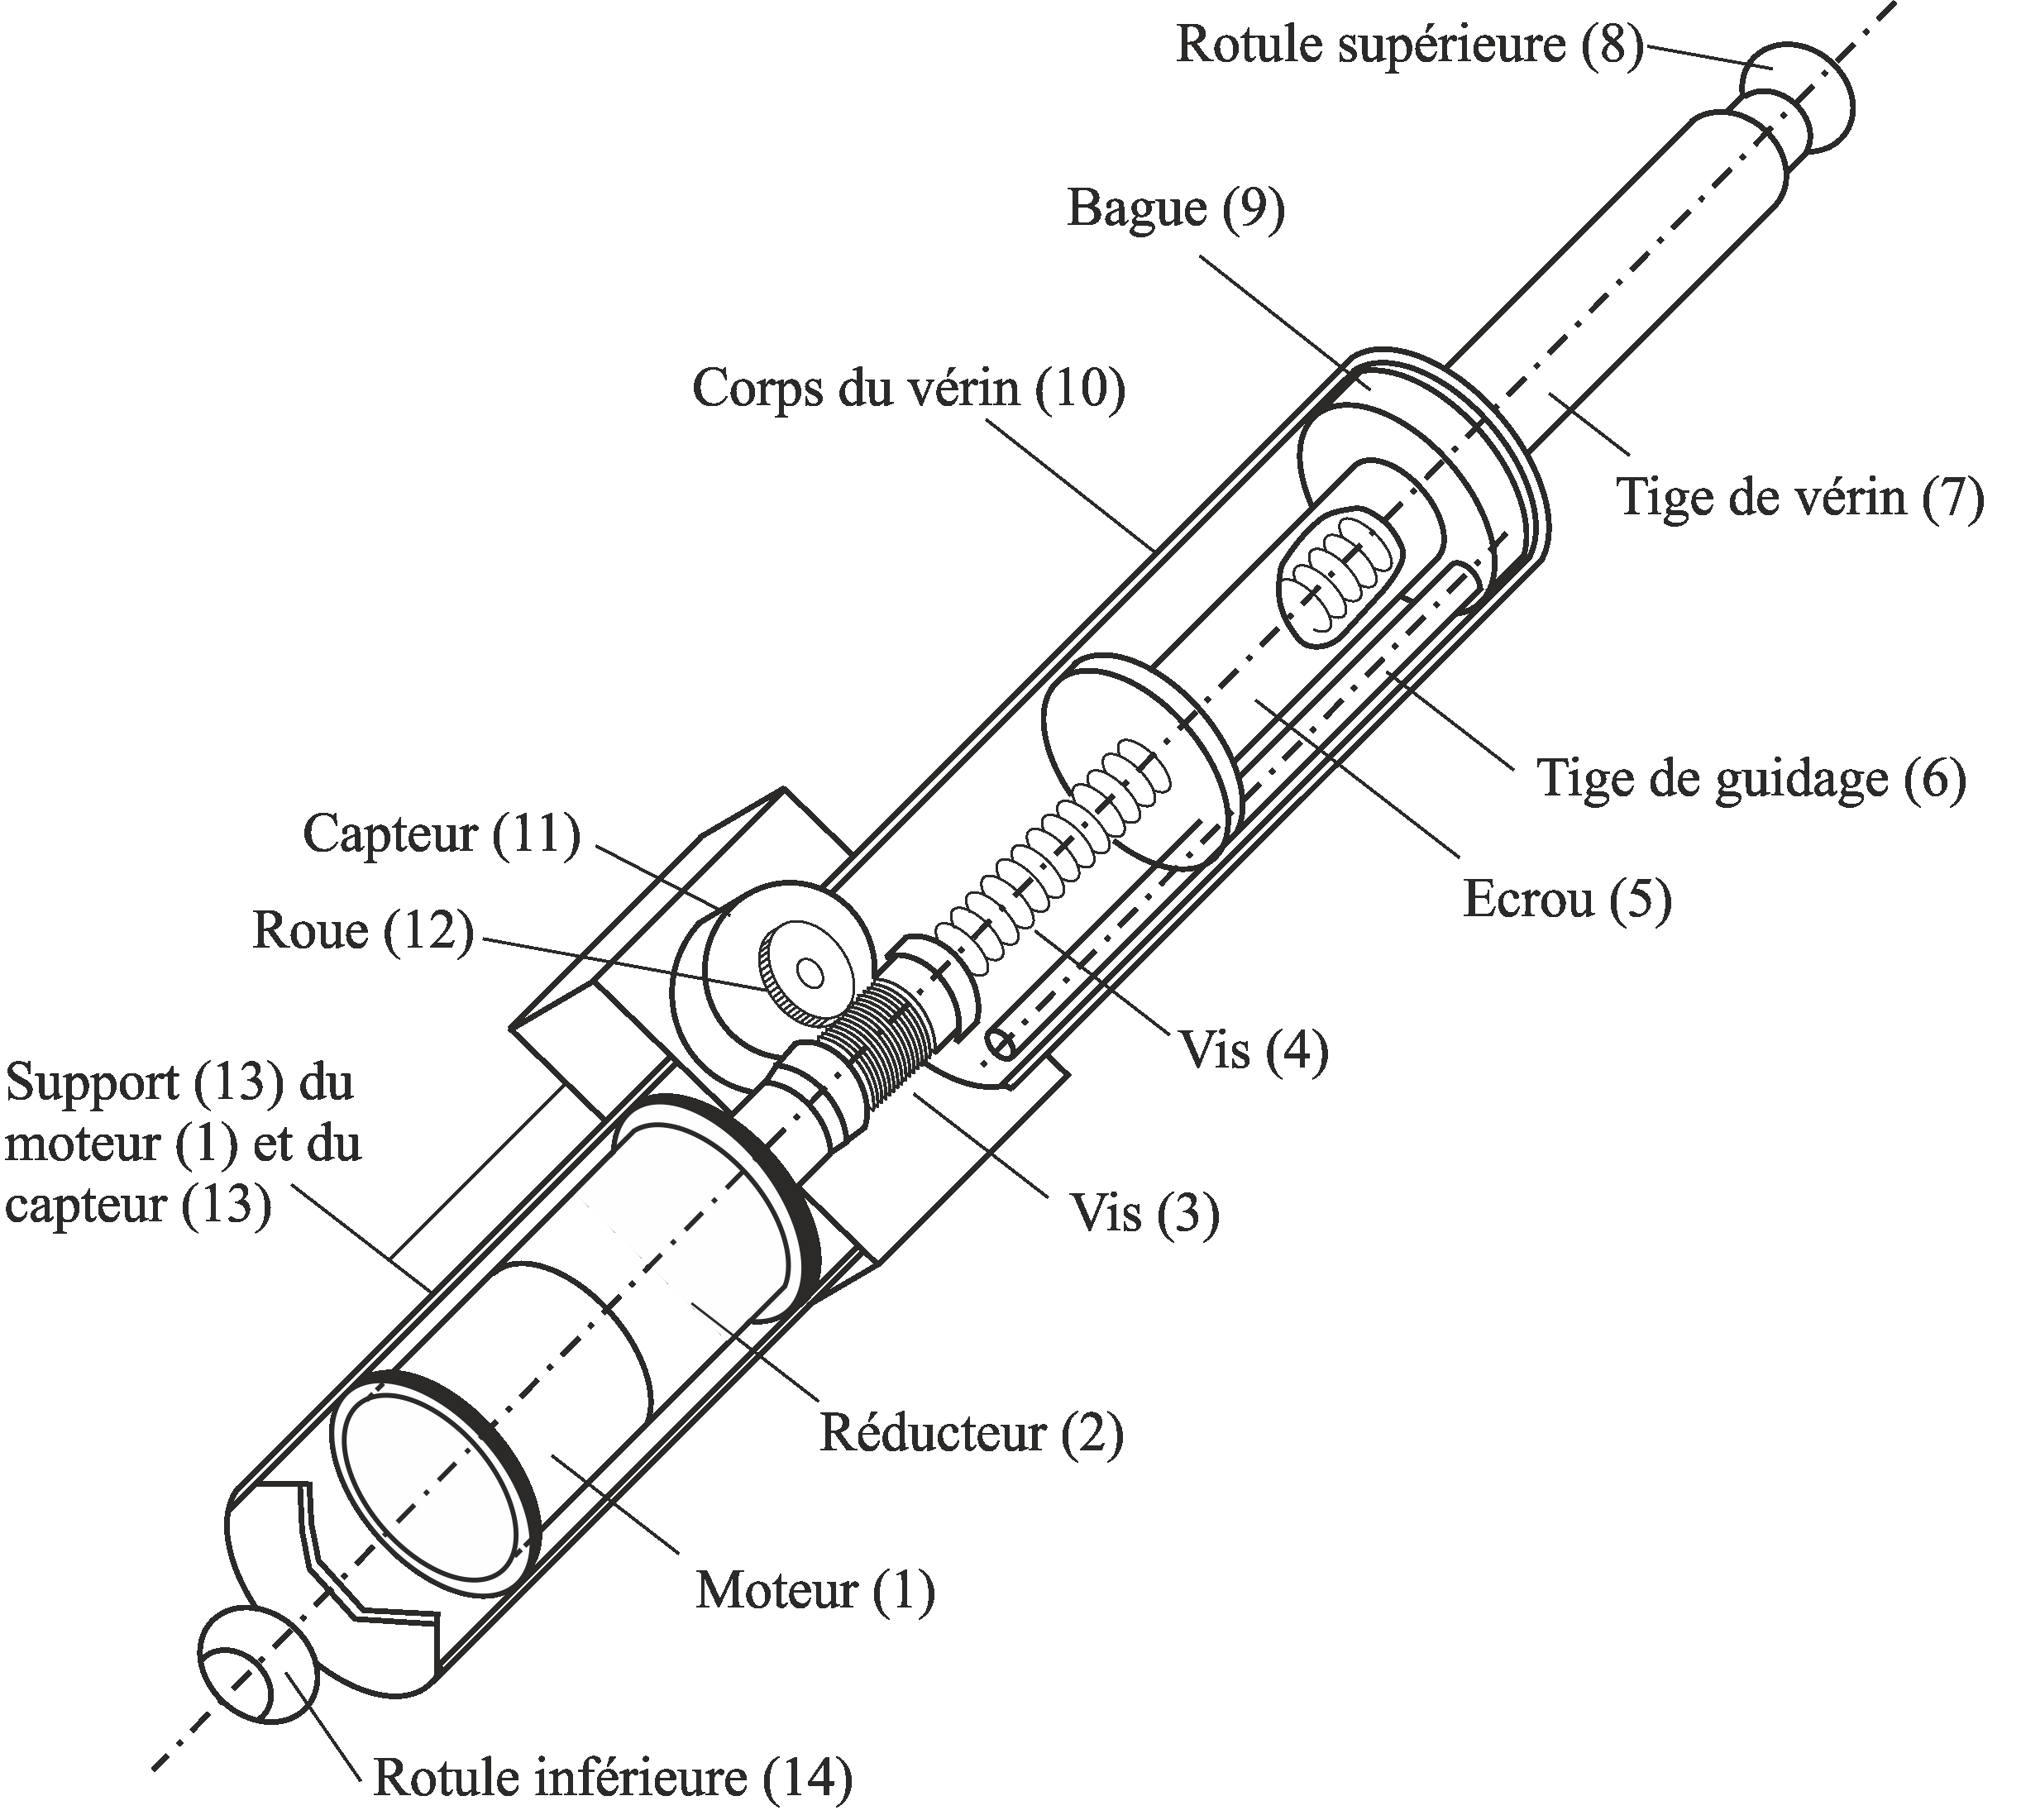
\includegraphics[width=.7\linewidth]{fig_04.png}
\caption{Principe du capteur de proximité \label{fig_04}}
\end{figure}

Ainsi au niveau du capteur de proximité, l’information exploitable est le temps $T_e$
entre l’émission et la réception
du signal (écho) émis par le capteur. C’est l’acquisition de $T_e$ qui servira dans l’algorithme pour l’identification
d’une place libre et pour la caractérisation de la trajectoire à suivre.

La \autoref{fig_05} représente le profil de vitesse du véhicule lorsque ce dernier longe une place libre. Le temps $T_a$
représente l’instant où le temps $T_e$ augmente brusquement (ce qui correspondrait au point $A$ \autoref{fig_03}). Le temps
$T_b$
correspond au moment où $T_e$ diminue brusquement (ce qui correspondrait au point B \autoref{fig_03}).

\begin{figure}[H]
\centering
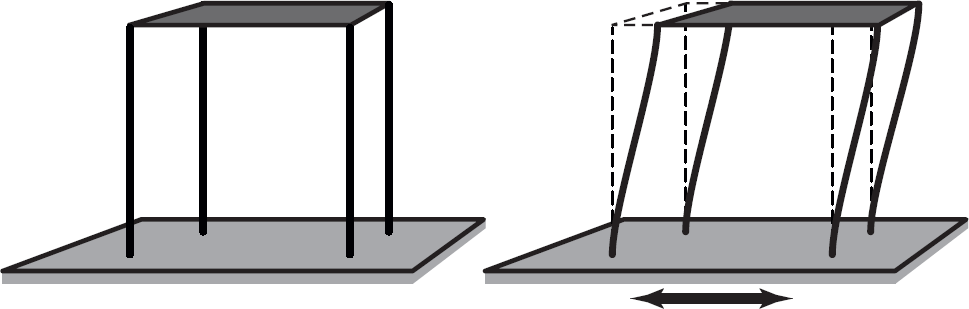
\includegraphics[width=.7\linewidth]{fig_05.png}
\caption{Profil de vitesse du véhicule lors des phases 1, 2 et 3 de la figure \ref{fig_05} \label{fig_05}}
\end{figure}

Lors de la phase de détection le véhicule avance à une vitesse $V_d$ constante et connue (information déduite de
capteurs situé au niveau des roues). La longueur du véhicule notée $L_v$
est également connue comme tous les
paramètres géométriques du véhicule.

Le fait de relever $\Delta T_p = T_b - T_a$ au niveau du capteur \textbf{a} permet de déterminer la longueur de la place et de vérifier qu’elle est compatible avec la manœuvre.

\question{Déterminer la condition que la grandeur $\Delta T_p$ doit vérifier pour que la longueur $L$ d’une place de stationnement respecte l’exigence 1.4. Cette condition est fonction de $V_d$ et $L_v$.}

Lorsque la voiture longe la place libre (entre les repères A et B \autoref{fig_03}), c’est la valeur maximale de $T_e$ relevée
lors du déplacement qui permet de savoir si la largeur de la place est suffisante pour la manœuvre. Cette largeur
est notée $e$ (\autoref{fig_03}) et la largeur du véhicule est notée $e_v$. La grandeur $D$ désigne la distance latérale par rapport aux véhicules déjà stationnés (\autoref{fig_03}).

\question{Déterminer la condition sur le temps $T_e$ pour que la largeur d’une place de stationnement respecte
l’exigence 1.4.}

Les conditions de longueur et de largeur d’une place de stationnement étant vérifiées, les distances $L$ et $e$ étant déduites des mesures, ces deux dernières grandeurs sont désormais des données implantables dans l’algorithme de stationnement. Le fait de connaitre en temps réel la vitesse du véhicule donne aussi la possibilité de connaitre la position du véhicule à partir d’un instant de référence tel que $T_a$. Il est donc maintenant considéré que la
position du point $A$ par rapport au véhicule est une donnée.

Une place de stationnement libre étant acceptée pour la manœuvre et sa géométrie (longueur, largeur, position
des obstacles) étant connue, il reste à caractériser la trajectoire à suivre pour la manœuvre.

\subsection{Trajectoire à suivre pour le stationnement (exigence 1.2)}

\begin{obj}
L’objectif est de déterminer les paramètres géométriques à implanter dans l’algorithme de stationnement afin d’y définir la trajectoire à suivre pour le stationnement.
\end{obj}

\subsubsection{Caractérisation de la trajectoire à suivre}
Une fois que le véhicule a longé une place et qu’il est à l’arrêt (position 3 \autoref{fig_02}) la manœuvre de type créneau
débute par une phase de recul rectiligne jusqu’à ce que le train arrière soit au niveau de l’extrémité arrière du
véhicule déjà stationné (point $B$ \autoref{fig_06}). Toujours en recul, il s’en suit le braquage des roues (dans un sens
puis l’autre) pour l’insertion dans la place libre.

La trajectoire du véhicule est définie par celle du point $F$, centre du train arrière (\autoref{fig_06}). La trajectoire
« idéale » de $F$ est donc une portion linéaire jusqu’au point $O$ suivie de deux arcs de cercles identiques (sur les cercles $C_1$ et $C_2$) tangents en un point $P$. Ce dernier est le point où le véhicule fait un angle de 45\degres par rapport
au trottoir.

Le point $O$ est défini à partir de la longueur $L$  de la place de stationnement, des dimensions du véhicule et de
la distance $D$ de ce dernier avec le véhicule déjà stationné en amont de la place libre.

Le \autoref{tab_01} précise les paramètres géométriques qui caractérisent la trajectoire du véhicule pendant la manœuvre de stationnement.

\question{Parmi tous les paramètres géométriques définis dans le \autoref{tab_01} ainsi que sur la \autoref{fig_06}, identifier
ceux qui sont propres au véhicule et ceux qui se déduisent directement des informations des capteurs à ultrasons.
Que reste-t-il donc à déterminer afin que la géométrie de la trajectoire du point $F$ soit définie ?}

\begin{figure}[H]
\centering
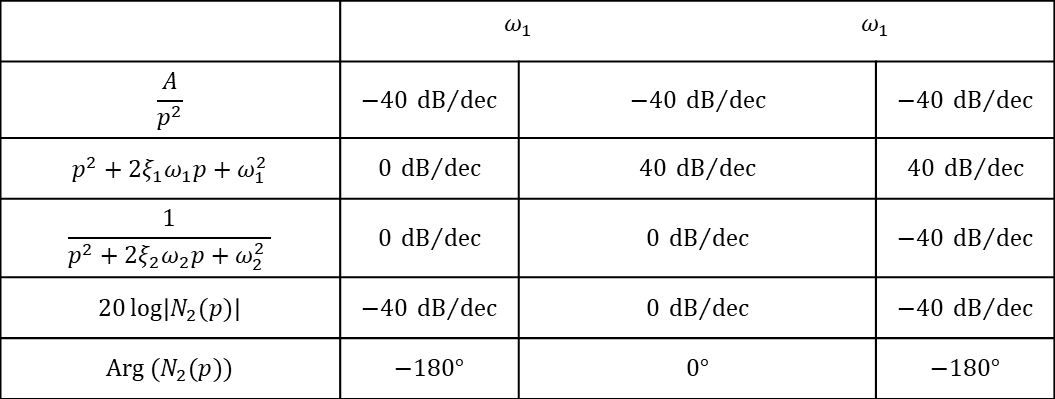
\includegraphics[width=\linewidth]{fig_06.png}
\caption{Trajectoire à suivre pour la manoeuvre \label{fig_06}}
\end{figure}

\begin{table}
\begin{itemize}
\item Paramètres de la place de stationnement :
\begin{itemize}
\item $L$ longueur de la place libre ;
\item $e$ largeur de la place libre.
\end{itemize}
\item Autres paramètres géométriques :
\begin{itemize}
\item $D$ distance latérale par rapport au véhicule déjà stationné ;
\item $L_F$ distance train arrière/extrémité arrière du véhicule ;
\item $R$ rayon des cercles $C_1$ et $C_2$ composant la trajectoire ;
\item $L_a$ distance entre l’arrière du véhicule en manœuvre et du véhicule placé derrière ;
\item $e_v$ largeur du véhicule en manœuvre ;
\item $d_r$ distance latérale entre le véhicule stationné et tout obstacle limitant la largeur de la place de stationnement.
\end{itemize}
\end{itemize}
\caption{Définition des paramètres géométriques qui caractérisent la trajectoire \label{tab_01}}
\end{table}

\begin{itemize}
\item $\rep{0} \repere{O}{x_0}{y_0}{z_0}$ est un repère défini au point $O$. 
\item Les points $O_1$ et $O_2$ sont respectivement les centres des cercles $C_1$ et $C_2$.
\item Le point $P$ est milieu de $[O_1 O_2]$.
\item Les cercles $C_1$ et $C_2$ sont de même rayon $R$.
\item La position du point $F$ est repérée par un angle $\theta_1(t)$ (\autoref{fig_07}) dans le repère
$\repere{O_1}{x_0}{y_0}{z_0}$ et par un angle $\theta_2(t)$ (\autoref{fig_07}) dans le repère $\repere{O_2}{x_0}{y_0}{z_0}$.
\item Le point $F_0$ correspond à la position initiale du point $F$ et $F_f$ à celle de la position finale lors de la phase d’insertion.
\end{itemize}


\begin{figure}[H]
\centering
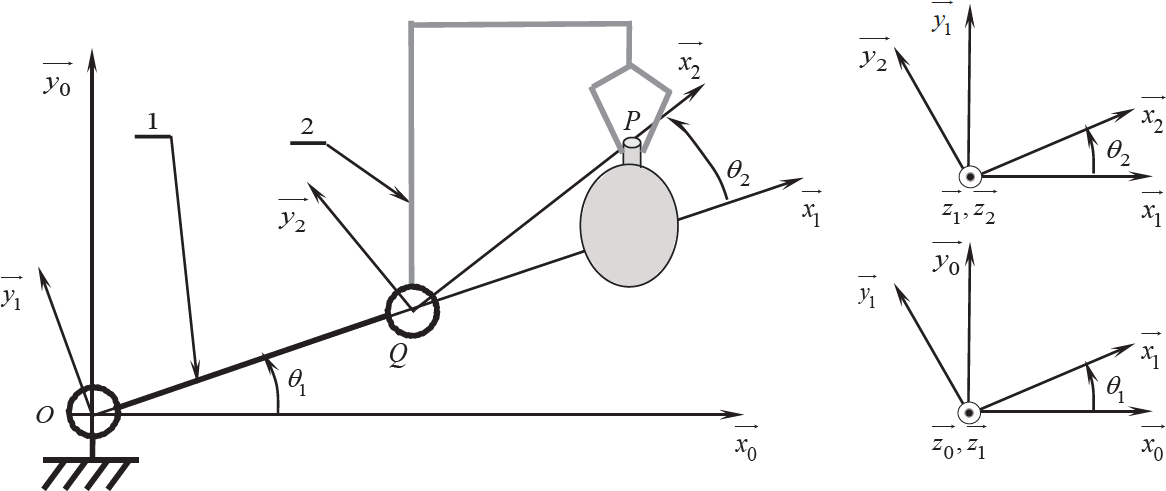
\includegraphics[width=.75\linewidth]{fig_07.png}
\caption{Trajectoire du point $F$ lors de l’insertion dans la place vacante \label{fig_07}}
\end{figure}

%Q5
\question{Les coordonnées du point $P$ dans le repère $\rep{0}$ sont notées $x_p$
et $y_p$ : $\vect{OP}=x_P\vect{x_0}+y_P\vect{y_0}$. Déterminer
l’expression de $x_P$ et $y_P$ en fonction des paramètres géométriques $L$, $e$, $L_F$, $d_r$, $L_a$ et $D$. Le rayon $R$ n’étant pas encore déterminé, il ne doit pas apparaitre dans les expressions de $x_P$ et $y_P$.}

%Q6
\question{Déterminer l’expression de $R$ en fonction de $L$, $L_a$ et $L_F$ qui permettra de définir le cercle $C_1$ (et donc le cercle $C_2$).}

Le cercle $C_1$ (et donc $C_2$ par symétrie) est maintenant défini, donc la trajectoire que le point $F$ devra suivre l’est également.

Afin de vérifier en simulation la validité de la trajectoire déterminée, il est nécessaire de déterminer les coordonnées du point $F$ lors du déplacement du véhicule en insertion dans la place de stationnement.

\subsubsection{ Simulation et validation de la trajectoire à suivre}
%Q7
\question{Exprimer dans $\rep{0}$ les coordonnées $x$ et $y$ du point $F$ parcourant la portion de cercle $C_2$ en fonction de $R$ et $\theta_2$ : $\vect{OF}=x\vect{x_0}+y\vect{y_0}$. Préciser l’intervalle dans lequel $\theta_2$ doit varier.}

Le rayon $R$ et les coordonnées du point $F$ étant déterminés, il est maintenant possible d’implanter dans l’algorithme de stationnement le modèle de la trajectoire à suivre. Il est cependant nécessaire de valider la trajectoire
déterminée en prenant en compte l’ensemble du véhicule avant de poursuivre par l’étude de la direction du
véhicule.

En se servant de l’expression de $R$ et de celle des coordonnées du point $F$ lors du mouvement du véhicule, il est
possible de réaliser une simulation de la manœuvre d’insertion dans la place envisagée.
La \autoref{fig_08} représente le résultat de cette simulation. Le nombre de positions du véhicule représentées a été limité
à quatre par souci de clarté. La simulation a été réalisée pour une voiture dont les dimensions correspondent
à la moyenne des véhicules vendus en France et en prenant une place de stationnement compatible avec la
manœuvre. La trajectoire a été déterminée à partir des relations trouvées dans les études précédentes.

\begin{figure}[H]
\centering
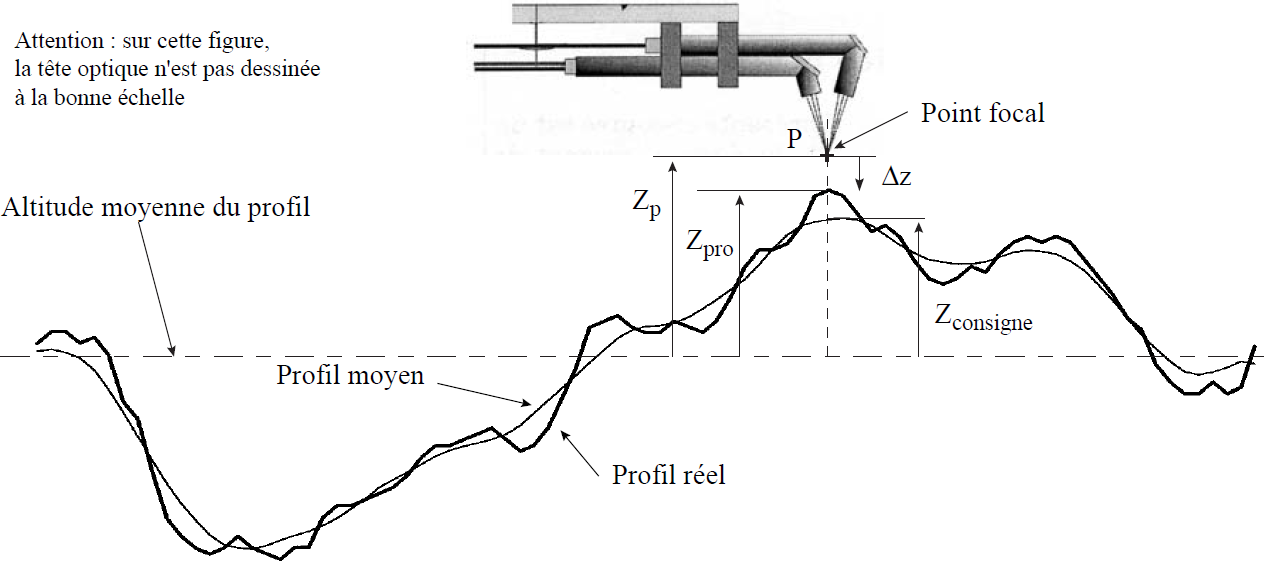
\includegraphics[width=.9\linewidth]{fig_08.png}
\caption{Simulation du stationnement \label{fig_08}}
\end{figure}

%Q8
\question{Quelles sont les exigences dimensionnelles vérifiées par la simulation (\autoref{fig_08}) et permettant de valider
la trajectoire ? Justifier les réponses apportées.}

La simulation a permis de valider la trajectoire à suivre. Cependant il faut encore établir le lien entre l’orientation
des roues directrices du véhicule et la trajectoire à suivre puisque le système de stationnement automatique agit
directement sur les roues directrices du véhicule.

\subsection{Direction du véhicule}

\begin{obj}
L’objectif est de déterminer la consigne angulaire des roues directrices du véhicule et sa vitesse de
recul lors de la phase d’insertion dans la place de stationnement.
\end{obj}


Pour l’étude il est choisi de prendre un véhicule type traction (roues avant motrices) comme 90\% des véhicules
vendus en France. De plus, la détermination de l’angle d’orientation des roues directrices (noté $\alpha$ sur la \autoref{fig_09})
sera limitée à la première portion de cercle $C_1$ pour laquelle le véhicule est en rotation autour du point $O_1$. Du
fait de la symétrie de la trajectoire, il n’est donc pas nécessaire de prolonger la détermination de $\alpha$ à la portion
de cercle $C_2$.

L’insertion du véhicule dans la place de stationnement peut se décomposer en trois phases à partir de l’instant
$t_0$ où le véhicule est à l’arrêt après avoir longé la place de stationnement envisagée.

\begin{itemize}
\item Phase 0 : recul rectiligne permettant au point $F$ d’atteindre le point $O$. La durée de cette phase est notée $\Delta T_0$.
\item Phase 1 : recul avec braquage des roues directrices, l’objectif étant que le point $F$ parcoure la portion de
cercle $C_1$ jusqu’au point $P$. La durée de cette phase est notée $\Delta T_1$.
\item Phase 2 : recul avec contre-braquage des roues directrices, l’objectif étant que le point $F$ parcoure la portion
de cercle $C_2$ jusqu’au moment où le véhicule est dans l’alignement de la place de stationnement. Comme la
manœuvre de stationnement se fait à vitesse constante et que les portions de cercle $C_1$
et $C_2$ sont symétriques, alors la durée de cette phase vaut également $\Delta T_1$.
\end{itemize}
Lors des phases de stationnement et entre chaque changement d’orientation des roues directrices du véhicule,
le véhicule recule à une vitesse supposée constante $v$ telle que $\vectv{C}{V}{\rep{1}}=v\vect{x_r}$. Dans la notation
$\vectv{C}{V}{\rep{1}}=v\vect{x_r}$. 
Dans la notation $\vectv{C}{V}{\rep{1}}=v\vect{x_r}$ $V$ désigne le véhicule et $\rep{1}\repere{O_1}{x_0}{y_0}{z_0}$
le repère galiléen défini au point $O_1$.

Le paramètre angulaire $\theta_1 = \angl{x_0}{y_0}$ (\autoref{fig_07}) définit la position relative de la base $\base{x_v}{y_v}{z_v}$
par rapport à la base $\base{x_0}{y_0}{z_0}$. Ainsi $\vecto{V}{\rep{1}} = \dot{\theta_1}\vect{z_0}$.

La \autoref{fig_09} représente le véhicule lors de la phase 1 de la manœuvre de stationnement. Comme l’orientation des
roues directrices (roues avant) sont liées entre elles, il n’est pas nécessaire de prendre en compte les deux roues.
$\alpha$ désigne l’angle que fait la roue intérieure au virage (côté trottoir) par rapport au véhicule (\autoref{fig_09}).

 $\alpha = \angl{x_v}{x_r}=\angl{y_v}{y_r}$
 avec $\rep{r} \repere{C}{x_r}{y_r}{z_r}$ 
un repère orthonormé direct défini au point $C$, centre de la roue intérieure, et tel que $\axe{C}{y_r}$ est confondu avec l’axe de cette roue (\autoref{fig_09}) et $\rep{v}\repere{F}{x_v}{y_v}{z_v}$ un repère
orthonormé défini au point $F$ et lié au véhicule (\autoref{fig_09}).

\begin{figure}[H]
\centering
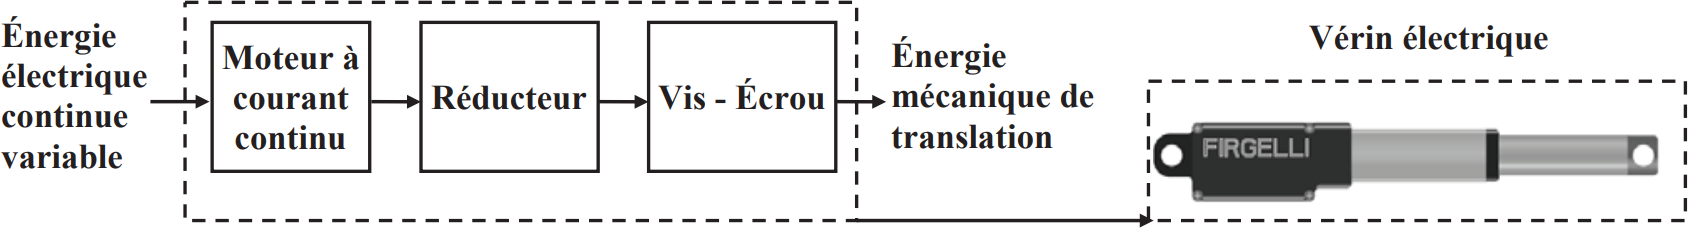
\includegraphics[width=.45\linewidth]{fig_09.png}
\caption{Paramétrage lors de la manoeuvre \label{fig_09}}
\end{figure}


\begin{figure}[H]
\centering
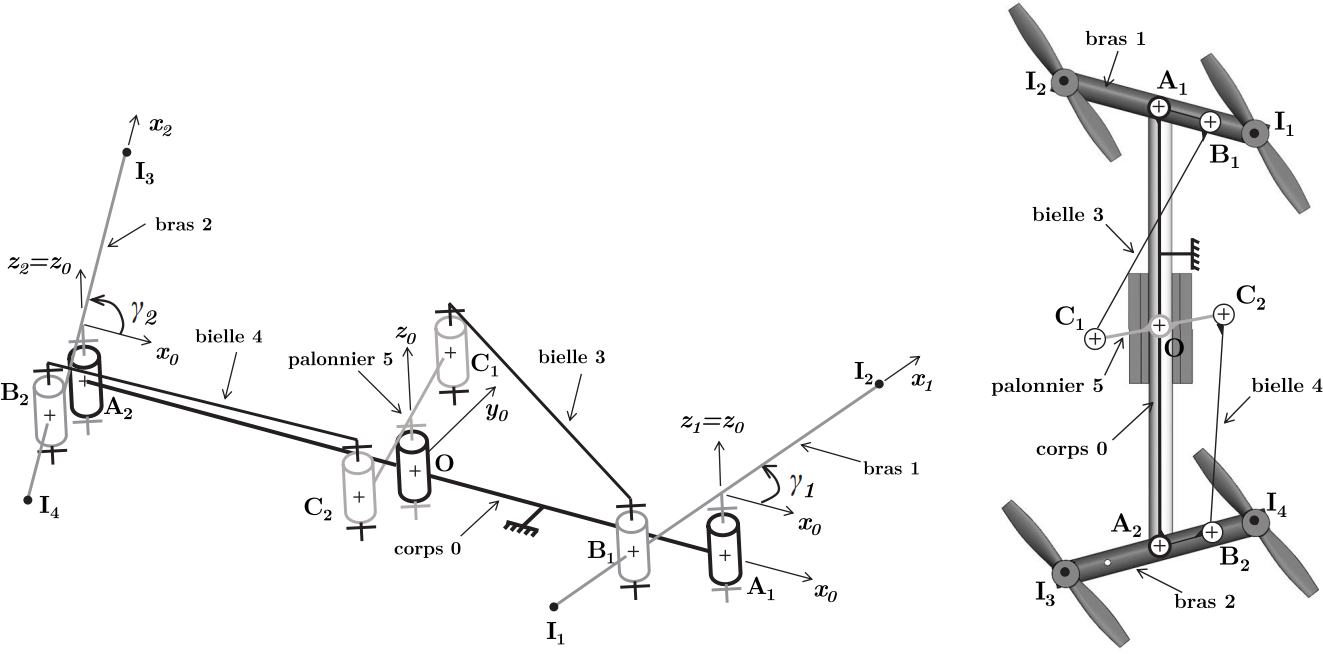
\includegraphics[width=.45\linewidth]{fig_10.png}
\caption{Tamiya M-05 Mazda \label{fig_10}}
\end{figure}


\begin{figure}[H]
\centering
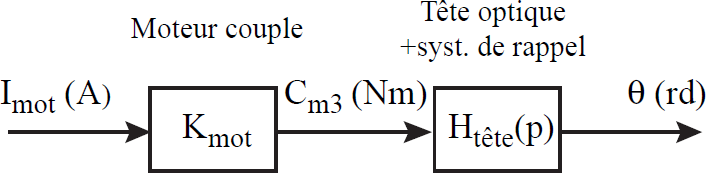
\includegraphics[width=.45\linewidth]{fig_11.png}
\caption{Description chaine d’énergie / chaine d’information de la direction \label{fig_11}}
\end{figure}


\begin{figure}[H]
\centering
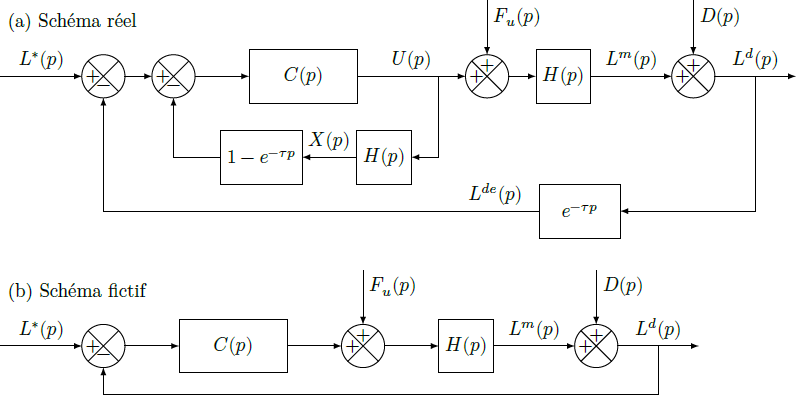
\includegraphics[width=.45\linewidth]{fig_12.png}
\caption{Schéma blocs de la commande en position des roues directrices du véhicule RC \label{fig_12}}
\end{figure}


\begin{figure}[H]
\centering
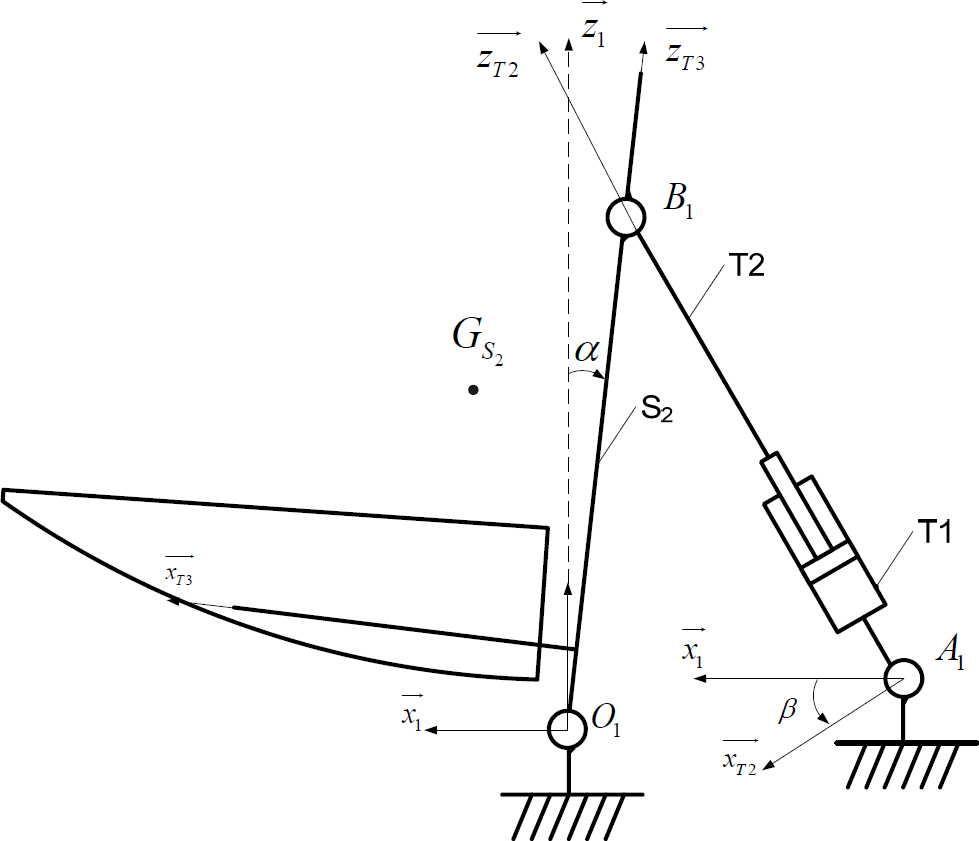
\includegraphics[width=.45\linewidth]{fig_13.png}
\caption{Schéma cinématique plan de la direction du véhicule radio commandé \label{fig_13}}
\end{figure}


\begin{figure}[H]
\centering
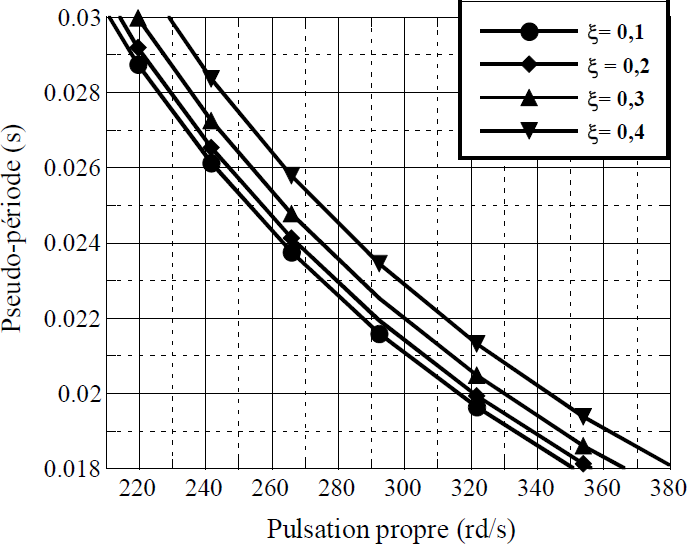
\includegraphics[width=.45\linewidth]{fig_14.png}
\caption{Schéma cinématique plan de la direction du véhicule radio commandé \label{fig_14}}
\end{figure}


\begin{figure}[H]
\centering
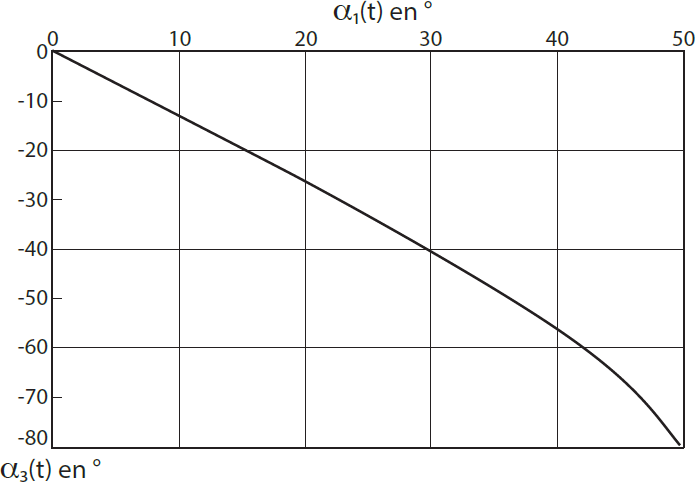
\includegraphics[width=.45\linewidth]{fig_15.png}
\caption{Tracé de $\alpha_3(t)$ en fonction de $\alpha_1(t)$ \label{fig_15}}
\end{figure}


\begin{figure}[H]
\centering
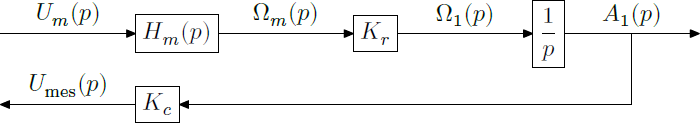
\includegraphics[width=.45\linewidth]{fig_16.png}
\caption{Schéma-blocs du servomoteur seul \label{fig_16}}
\end{figure}


\begin{figure}[H]
\centering
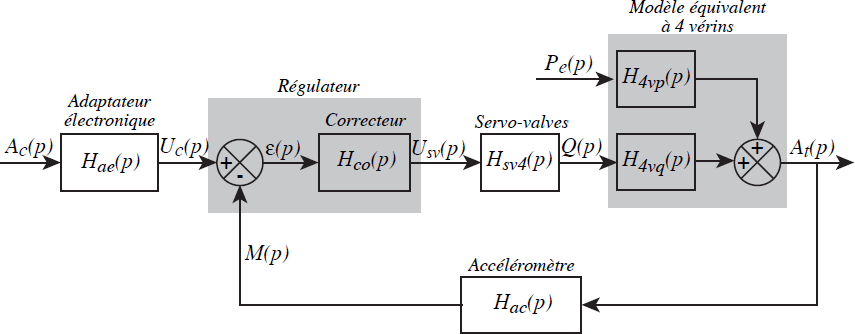
\includegraphics[width=.45\linewidth]{fig_17.png}
\caption{Tension fournie par le potentiomètre du servomoteur pour un échelon de tension $u_m(t)=\SI{3}{V}$ \label{fig_17}}
\end{figure}


\begin{figure}[H]
\centering
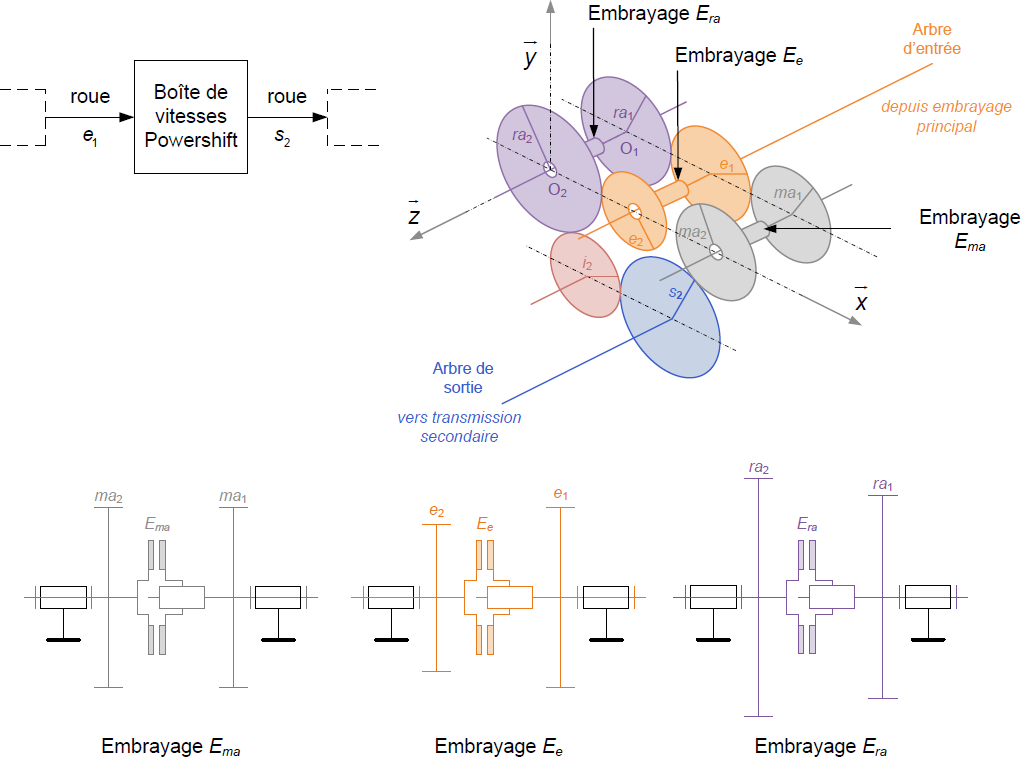
\includegraphics[width=.45\linewidth]{fig_18.png}
\caption{ Intensité moteur\label{fig_18}}
\end{figure}


\begin{figure}[H]
\centering
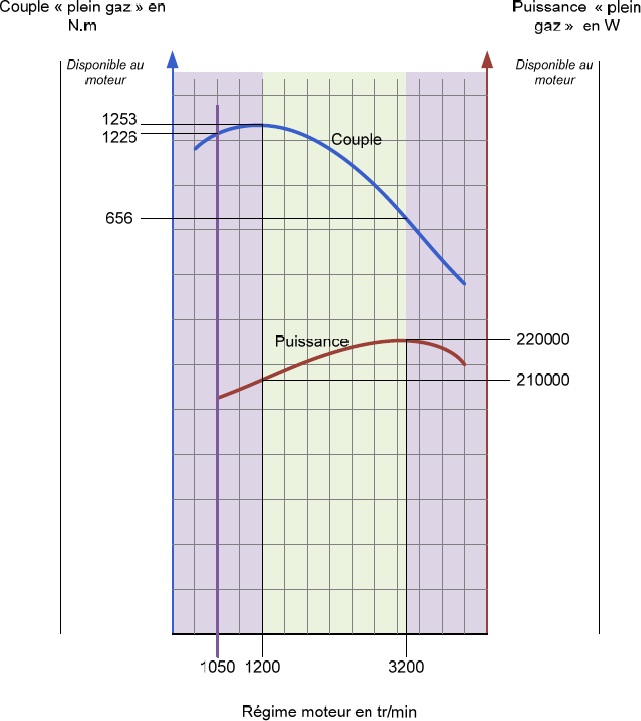
\includegraphics[width=.45\linewidth]{fig_19.png}
\caption{Acquisition de l’orientation des roues directrices \label{fig_19}}
\end{figure}


\begin{figure}[H]
\centering
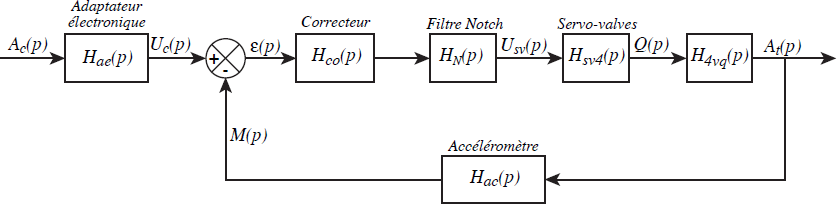
\includegraphics[width=.45\linewidth]{fig_20.png}
\caption{Schéma blocs de la commande en position des roues \label{fig_20}}
\end{figure}


\begin{figure}[H]
\centering
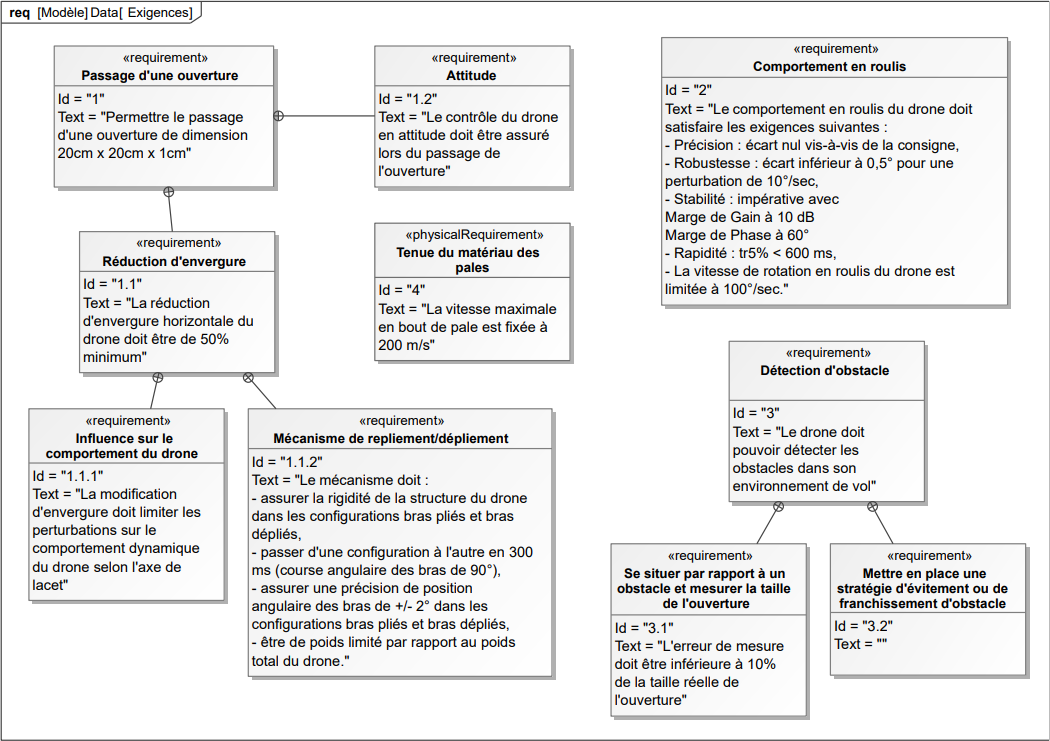
\includegraphics[width=.45\linewidth]{fig_21.png}
\caption{Évolution temporelle de $\alpha(t)$ pour une correction proportionnelle \label{fig_21}}
\end{figure}


\begin{figure}[H]
\centering
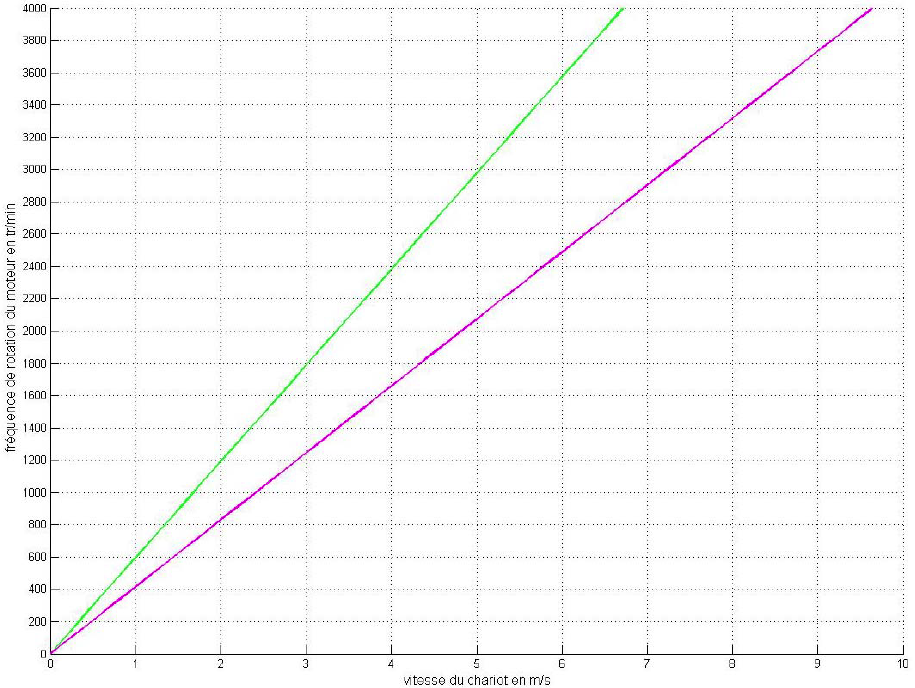
\includegraphics[width=.45\linewidth]{fig_22.png}
\caption{Essais expérimentaux réalisés sur le véhicule RC \label{fig_22}}
\end{figure}


\begin{figure}[H]
\centering
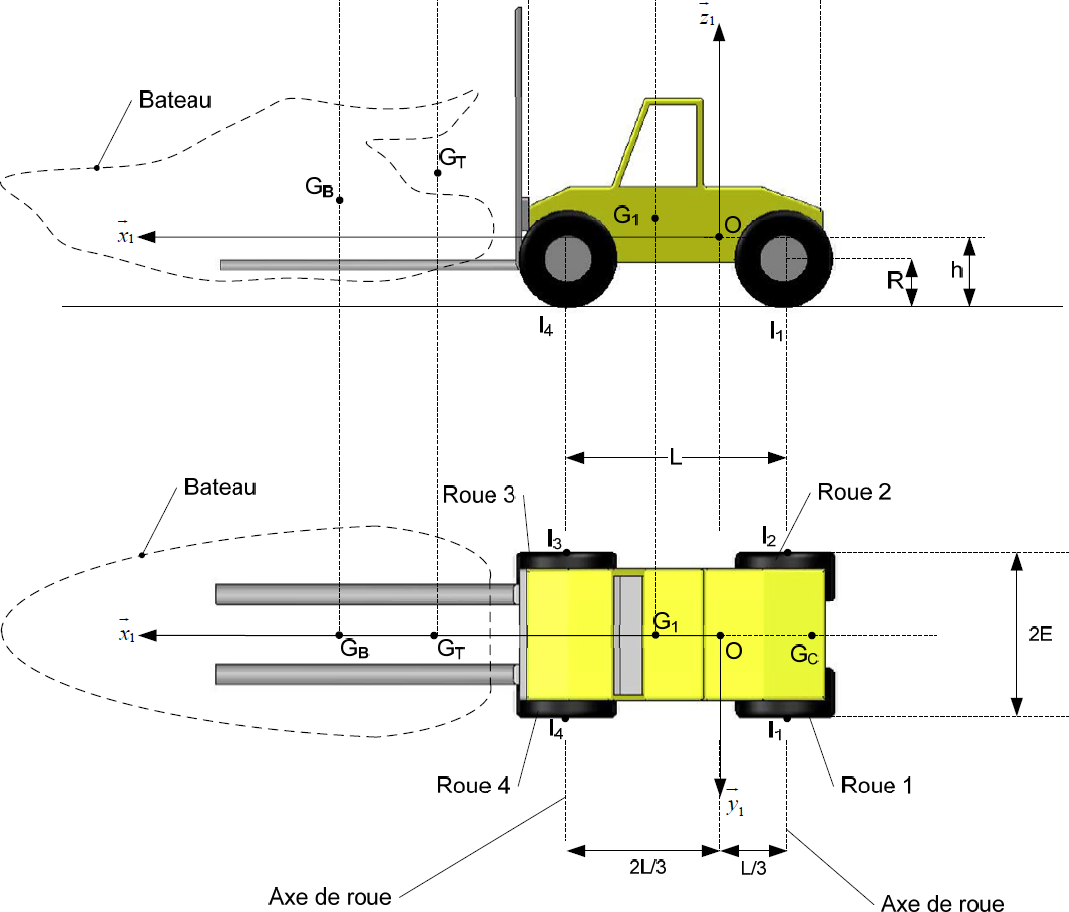
\includegraphics[width=.45\linewidth]{fig_23.png}
\caption{Diagrammes de Bode de la FTBO corrigée \label{fig_23}}
\end{figure}


\begin{figure}[H]
\centering
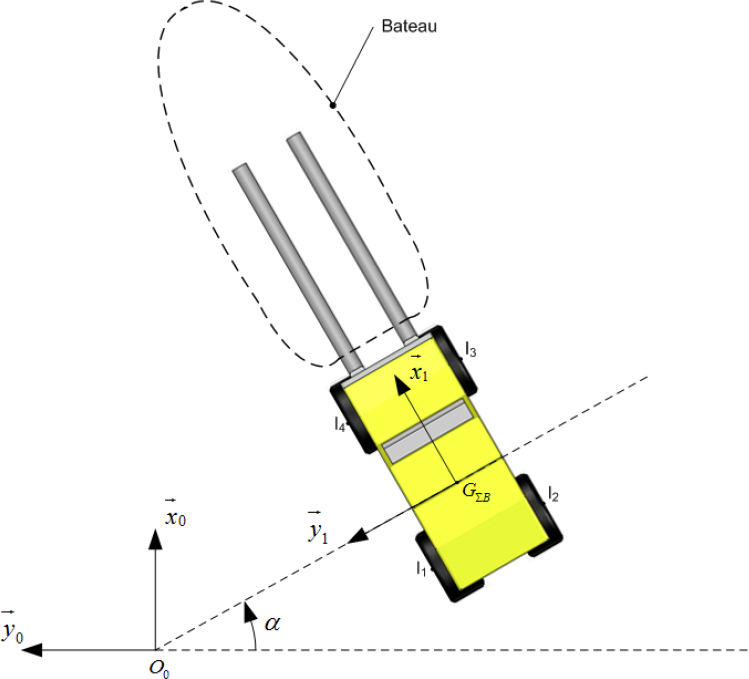
\includegraphics[width=.45\linewidth]{fig_24.png}
\caption{Angle des roues directrices \label{fig_24}}
\end{figure}


\begin{figure}[H]
\centering
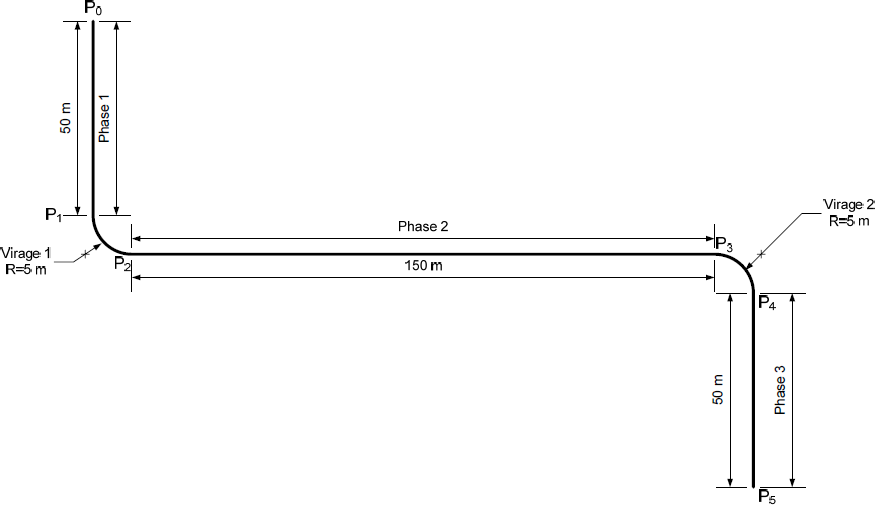
\includegraphics[width=.45\linewidth]{fig_25.png}
\caption{Résultat d’un essai de manoeuvre d’insertion avec l’algorithme d’aide au stationnement \label{fig_25}}
\end{figure}


\begin{figure}[H]
\centering
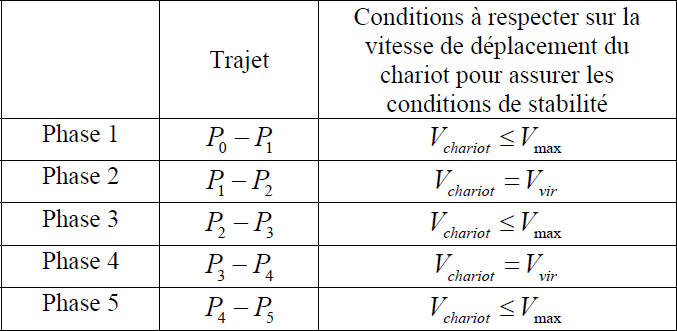
\includegraphics[width=.45\linewidth]{fig_26.png}
\caption{Extrait du diagramme des exigences du stationnement automatique \label{fig_26}}
\end{figure}


\begin{figure}[H]
\centering
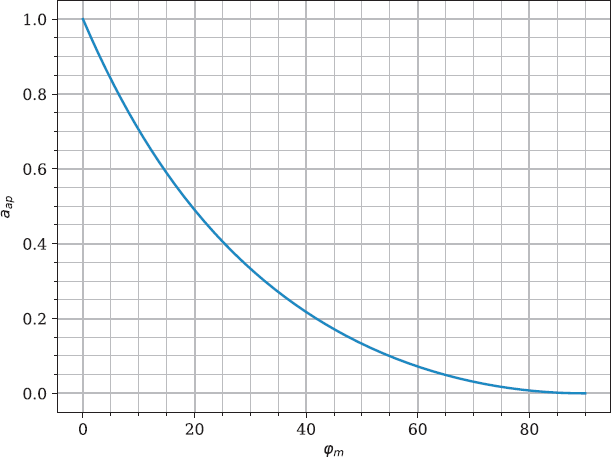
\includegraphics[width=.45\linewidth]{fig_27.png}
\caption{Extrait du diagramme des exigences du stationnement automatique \label{fig_27}}
\end{figure}


\begin{figure}[H]
\centering
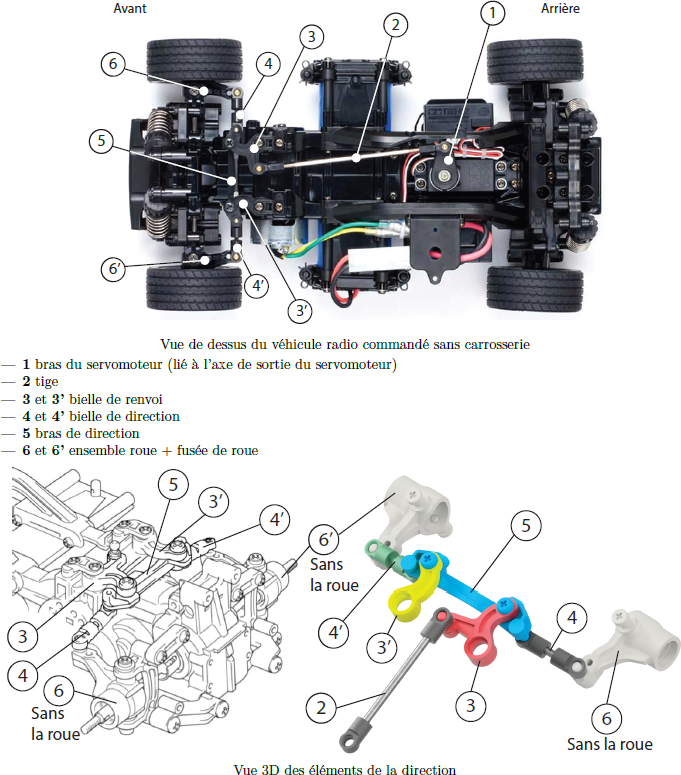
\includegraphics[width=.45\linewidth]{fig_28.png}
\caption{Description de la direction du véhicule radio commandé \label{fig_28}}
\end{figure}


\begin{figure}[H]
\centering
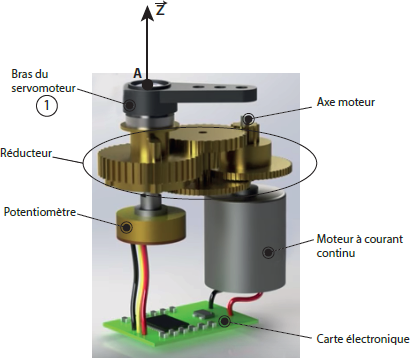
\includegraphics[width=.45\linewidth]{fig_29.png}
\caption{Composition du servomoteur \label{fig_29}}
\end{figure}